%%%------------------------------------------------------------------------------------------------------------
%%% 特征权重调优
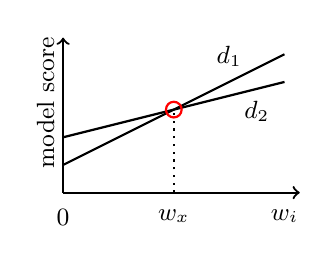
\begin{tikzpicture}
\begin{scope}
\node[anchor=west] (x0) at (0, 0) {};

\draw[->,thick] (x0.center) -- ([xshift=8.2em]x0.east);
\draw[->,thick] (x0.center) -- ([yshift=5.6em]x0.center);

{
\draw[thick] ([yshift=1em]x0.center) -- ([xshift=8em,yshift=5em]x0.center);
\draw[thick] ([yshift=2em]x0.center) -- ([xshift=8em,yshift=4em]x0.center);
\node[anchor=north] (e1) at ([xshift=6em,yshift=6em]x0.south) {\small{$d_1$}};
\node[anchor=north] (e2) at ([xshift=7em,yshift=4em]x0.south) {\small{$d_2$}};
\node[anchor=north,rotate=90] (e2) at ([xshift=-1.3em,yshift=3.6em]x0.south) {\small{model score}};
}

{
\node [anchor=center,draw=red,circle,inner sep=2pt,thick] (x1) at ([xshift=4em,yshift=3em]x0.center) {};
\draw[thick,dotted] ([xshift=4em]x0.center) -- ([xshift=4em,yshift=3em]x0.center);
}
\node[anchor=north] (zero) at ([yshift=0.1em]x0.south) {\small{0}};
\node[anchor=north] (wx) at ([xshift=4em,yshift=0.1em]x0.south) {\small{$w_x$}};
\node[anchor=north] (wi) at ([xshift=8em,yshift=0.1em]x0.south) {\small{$w_i$}};


\end{scope}
\end{tikzpicture}
